\documentclass{article}
\usepackage{graphicx} % Required for inserting images

\title{Notes on Bioelectric Signals and Electrodes}
\author{Arsh Arora}
\date{April 2023}

\begin{document}

\maketitle

\section{Introduction}
I am making this \LaTeX document and possibly a further series of notes for self-analysis and learning of various types of Biomedical Instruments.
\section{Origin of Bio-electric Signals}
The history of bio electric signals getting related to the human body has been in play since 18th Century when Galvani demonstrated it. The main sources of these signals are the muscles and nerves in our body. Potential changes also occur as a result of the electrochemical changes accompanied by the conduction of signals along with the nerves. Bio-electric potentials are generated at a cellular level and are the source of these potentials in ionic natures. The surrounding of these calls of the body are body fluids which are ionic and which provide a conducting medium for potentials. The membrane of excitable cells readily permits the entry of $K^+$ and $Cl^-$ but impedes the flow of $Na^+$. This leads to a higher concentration of $Na^+$ outside the cell when compared with inside.\\
\\
The unequal distribution of charge is a result of certain electrochemical reactions and processes occurring within the living cell and the potential measured is called a resting potential. The cell in such a condition is called polarised. A decrease in this resting membrane potential difference is called depolarisation.
Empirical evidence has shown that the resting potential within a cell is approximately $-90 mV$ with reference to the outside cell.\newpage
\begin{center}
    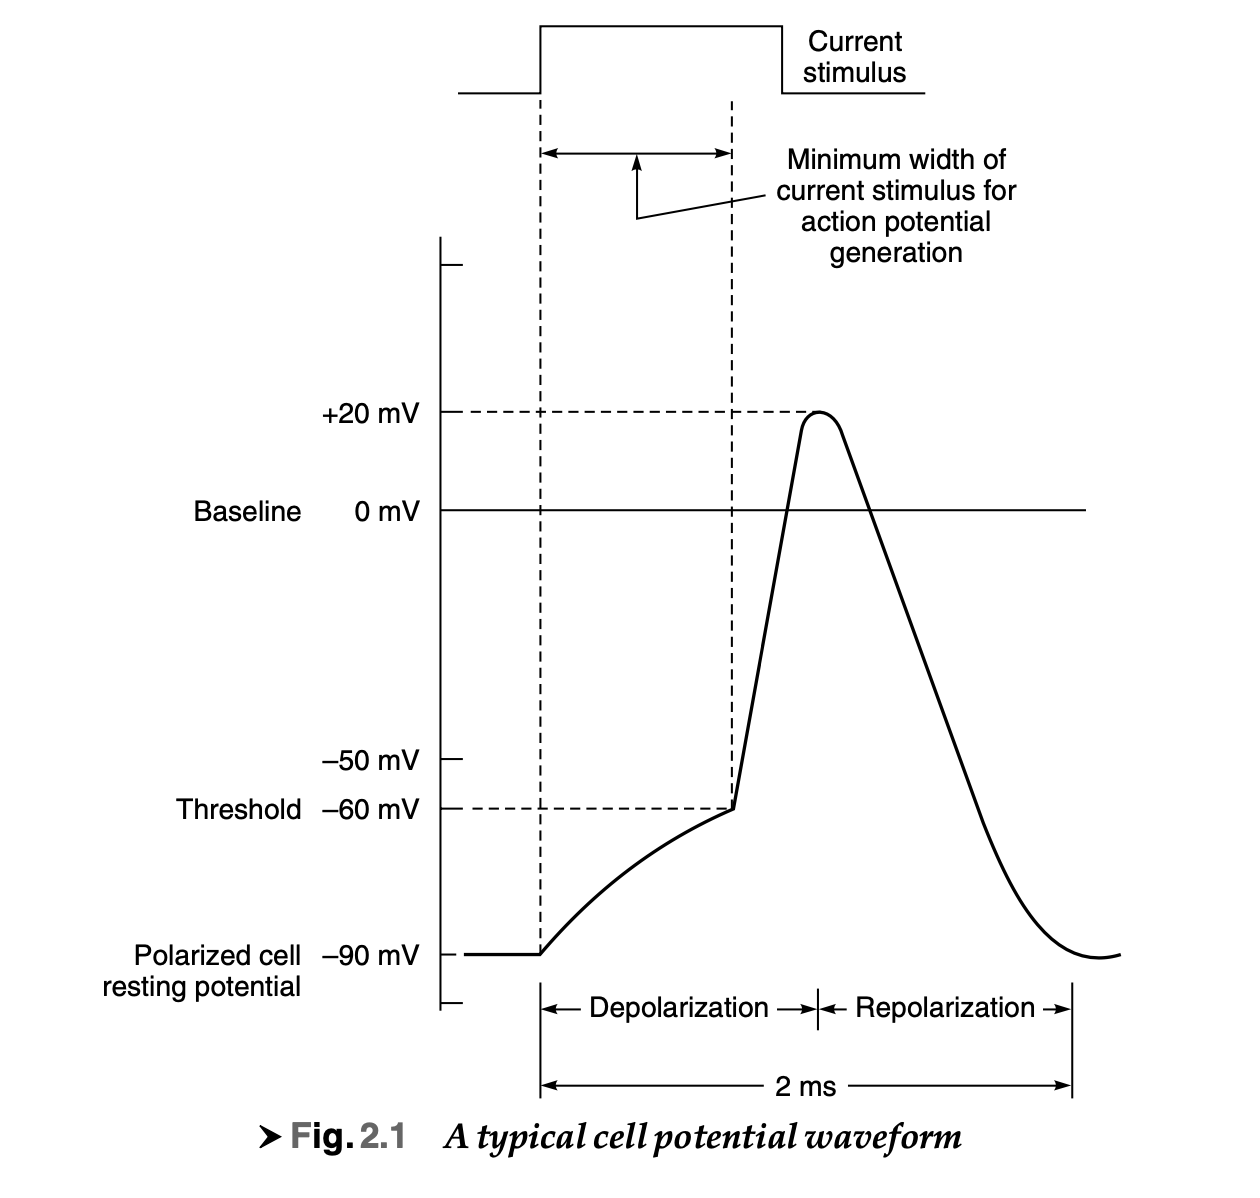
\includegraphics[scale=0.4]{Screenshot 2023-04-30 at 3.13.04 PM.png} 
    \\
    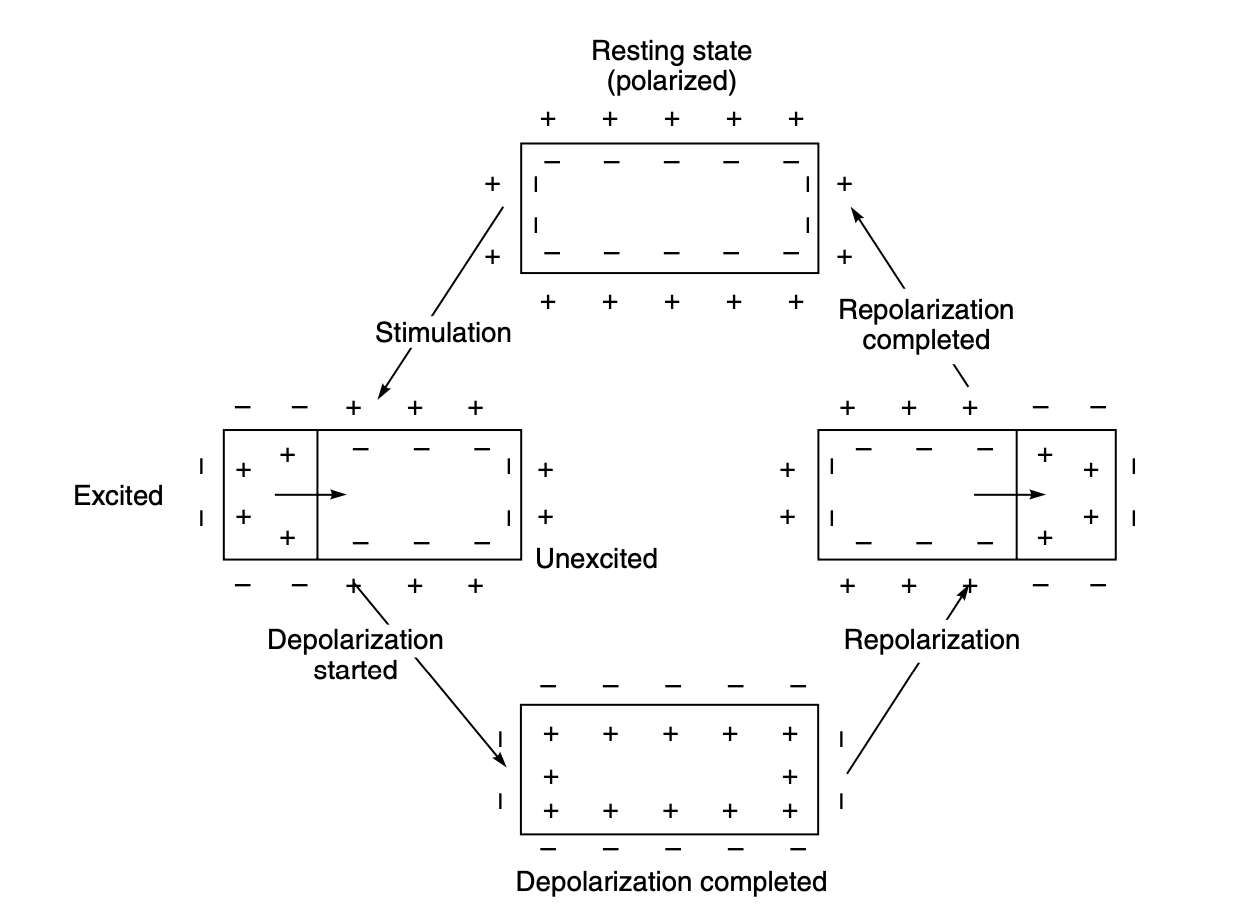
\includegraphics[scale=0.4]{Screenshot 2023-04-30 at 3.21.17 PM.png}
\end{center}
\begin{center}
    \begin{tabular}{|c|c|c|}
    \hline
        ECG & Frequency (0.05 to 120 $Hz$), Signal Amplitude (0.1 to 5$\mu V$) & Skin Electrodes  \\
        \hline
        EEG & Frequency (0.1 to 100 $Hz$), Signal Amplitude (2 to 200$\mu V$) & Scalp Electrodes \\
        \hline
        EMG & Frequency (5 to 2000 $Hz$), Signal Amplitude (0.1 to 5$\mu V$) & Needle Electrodes \\
        \hline
        ERG & Frequency (dc to 20 $Hz$), Signal Amplitude (0.5 to 1$\mu V$) & Contact Electrodes \\
        \hline
        EOG & Frequency (dc to 100 $Hz$), Signal Amplitude (10 to 3500$\mu V$) & Contact Electrodes \\
        \hline
    \end{tabular}
\end{center}\newpage
\subsection{Analysis of electrodes}
Electrodes basically act as an interface and transformer to convert the ionic conduction of muscles to electronic conduction which is vital for measurement.\\
\\ There are basically two types of electrodes used for measurement, they are
\begin{enumerate}
    \item Patient-Surface Electrodes
    \item Deep-Seated Electrodes
\end{enumerate}
The surface electrodes pick up signals from the surface and do not damage the live tissue, while the deep seated electrodes pick up the signal from deep inside the live tissue or cell. A major factor we should consider while picking an electrode is that it should be comfortable to wear a long period of time.
\subsection{Electrode Tissue Interface}
The Electrode-Tissue interface is basically comprised of two parts, which is the Metal-Electrolyte Interface and the Electrolyte-Skin Interface.
\subsubsection{Metal-Electrolyte Interface}
There is a tendency for each electrode to discharge ions in the electrolyte to combine with each electrode. The result of this is the creation of a charge gradient at each electrode, leading to the formation of the \textit{Electrical Double Layer.}\\
\\
The double layer is known to be present in the region immediately adjacent to the electrode and can be represented as two parallel sheets of charge of opposite sign separated by a thin film of dielectric. Therefore, the metal electrolyte interface appears to consist of a voltage source in series with a parallel combination of a capacitance and reaction resistance. The voltage developed is called the half-cell potential.\\When comparing the potential of electrodes, we take hydrogen absorbed on platinum to be the reference point of calculation.\newpage
\begin{table}
    \centering
    \begin{tabular}{|c|c|c|}
    \hline
        Metal & Ionic Symbol & Electrode Potential  \\
        \hline
        Aluminium & $Al^{+++}$ & -1.66 V \\
        Iron & $Fe^{++}$ & -0.44 V \\
        Lead & $Pb^{++}$ & -0.12 V \\
        Hydrogen & $H^{+}$ & 0 V \\
        Copper & $Cu^{++}$ & 0.34 V \\
        Silver & $Ag^{+}$ & 0.8 V \\
        Platinum & $Pt^{+}$ & 1.2 V \\
        Gold & $Au^{+}$ & 1.69 V \\
        \hline
    \end{tabular}
   \begin{center}
       \textbf{Electric potential of some commonly used electrode metals with Hydrogen}
   \end{center} 
    \label{tab:my_label}
\end{table}
The lowest potential observed in emperical studies was found to be in Silver-Silver Electrodes. The values of resistance and capacitance depend upon many factors which include the current density, temperature, type and concentration of the electrolyte and the type of metal used.\\The difference in the half cell potential of the two electrodes is also called as the offset potential. The every day amplifier designed to calculate the potential between two half cells, is design to cancel out the offset.
\\
When working with electrodes, we should also consider the relevance of electrolytes to be used in place so as to provide the least offset and use them healthily to get the best possible output.
\begin{center}
    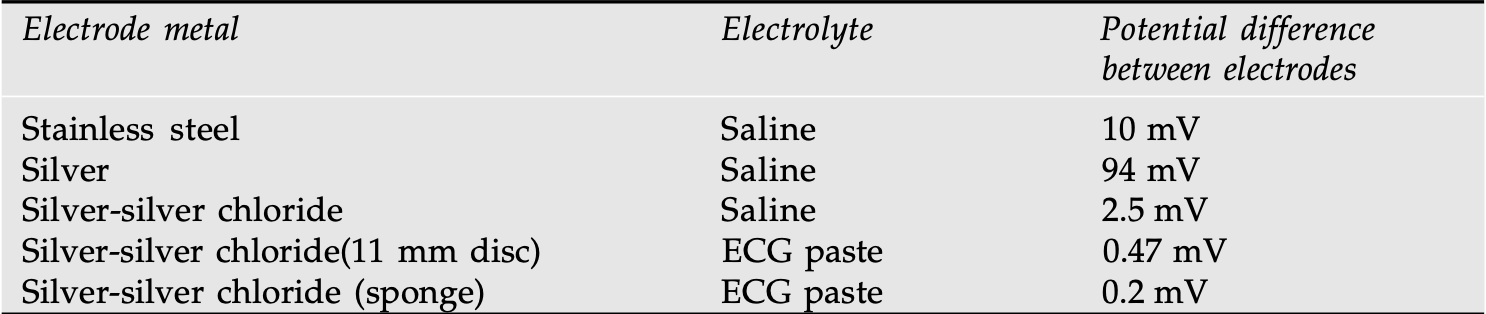
\includegraphics[scale=0.5]{Screenshot 2023-04-30 at 7.27.45 PM.png}
\end{center}
The above table clearly gives us a valid justification to not use stainless steel for electrodes in making.\\
Early hypothesis gave the recommendation of following the findings of Warburg regarding a thin electrolyte-electrode structure acting as an equivalent RC Circuit however analysis into the topic uncovered that it is only partially true and we need to consider a resistance in parallel which represents the Faradaic Leakage. This gives us an appropriate to study and base our calculations upon.
\begin{center}
    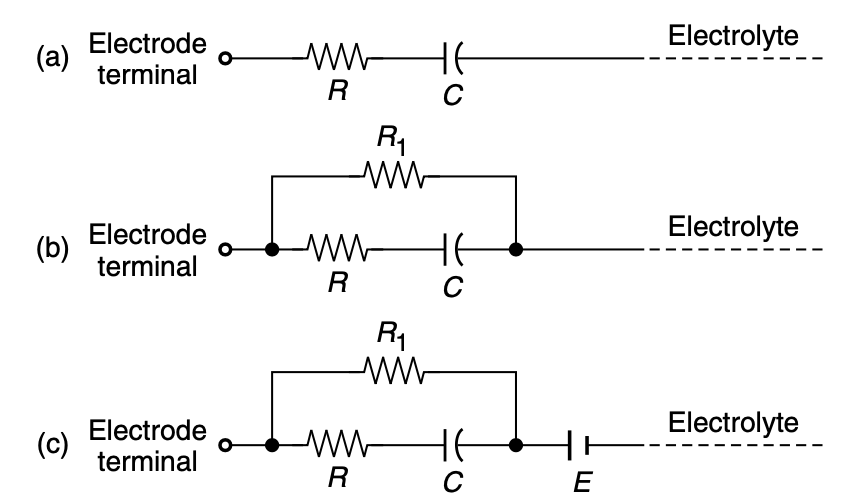
\includegraphics[scale = 0.5]{Screenshot 2023-04-30 at 7.38.55 PM.png}
\end{center}
\subsubsection{Electrolyte-Skin Interface}
An approximation of the electrolyte-skin interface can be had by assuming that the skin acts as a diaphragm arranged between two solutions (electrolyte and body fluids) of different concentrations containing the same ions, which is bound to give potential differences.\\The electrical equivalent of the circuit suggests that the voltage presented to the measuring instrument from the electrodes consists of two main components. One is the contact potential and the other is the biological signal of interest. The contact potential is found to be a function of the type of skin, skin preparation and composition of the electrolyte. When bio electric events are recorded, interference signals are produced by the potential differences of metal-electrolyte and the electrolyte-skin interference. \\
\\
If AC signal are to be recorded, the potential difference between the two electrodes will not interfere with the useful signals, provided that the contact potential difference between the electrodes is constant. However, if the rate of change with time of the contact potential falls within the frequency of the spectrum of the signal under the test an error will be produced. This problem raises to a higher level of severity when we discuss the working of EOG as it gives out a DC output.\\
\\
Based on aforementioned considerations, it is possible to construct the circuit in which a pair of electrodes is placed in electrolytic contact with a subject.The eventual circuit diagram of the electrodes would look like this at the end.\\
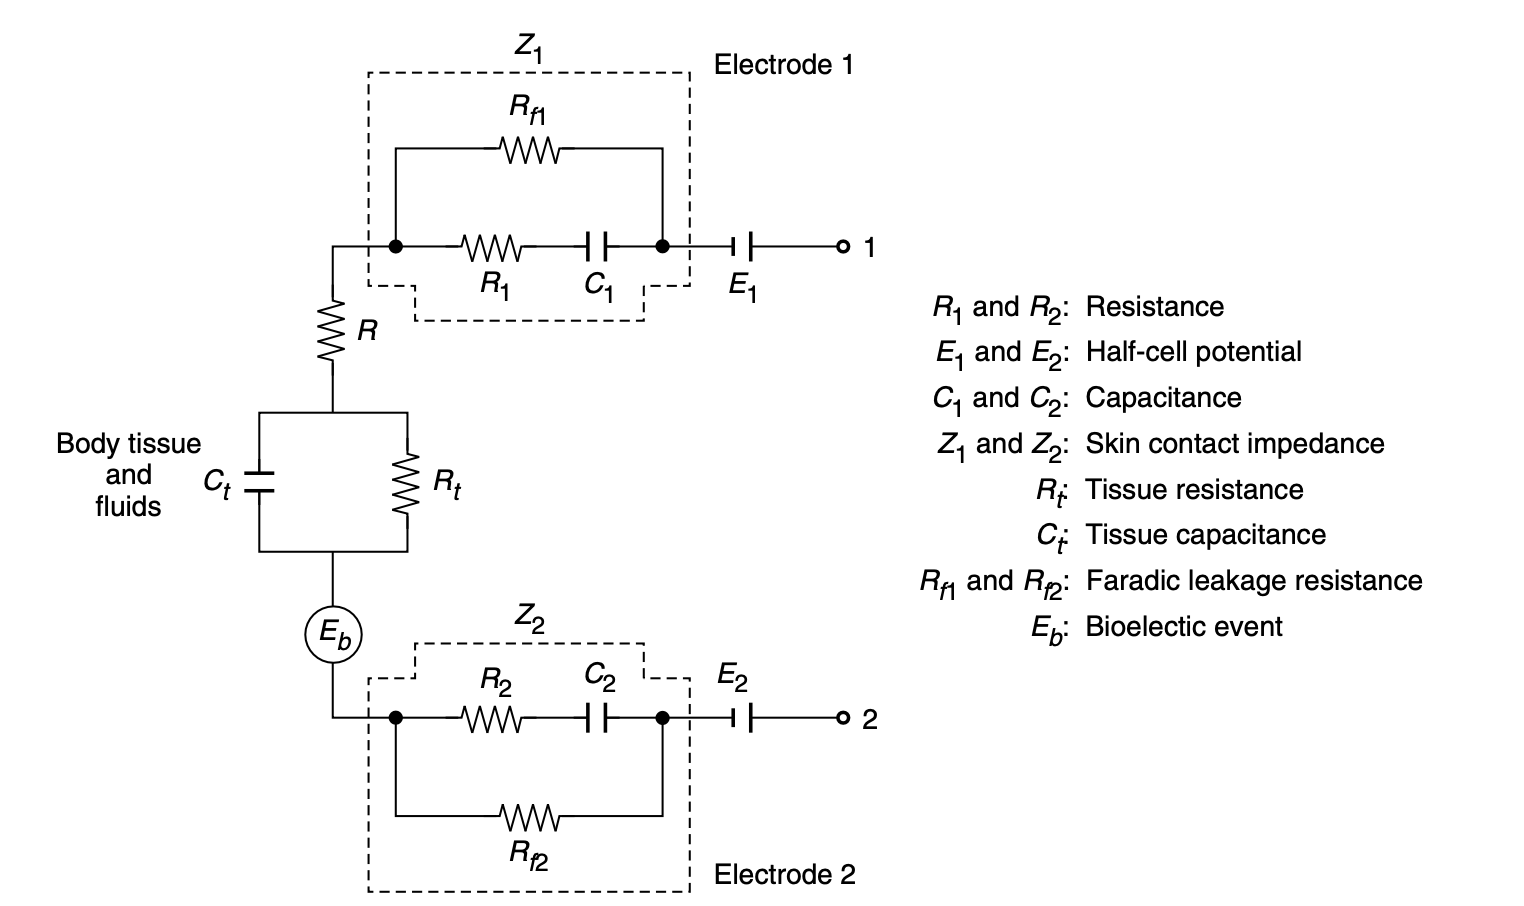
\includegraphics[scale=0.5]{Screenshot 2023-05-01 at 1.07.23 AM.png}
\\
\\There are three potentials found to exist as a whole, out of which one is bio electric, the other two are non physiological potentials and represent half cell potentials $E_1$ and $E_2$. $Z_1$ and $Z_2$ are the skin contact impedance of the electrodes and R is the tissue resistance.
\subsection{Polarisation}
Basically two types of electrodes exist, polarising and non polarising. Polarising vectors are mainly made using stainless steel and are used in cases when there is a small likely hood that the electrode will be exposed to a large pulse of energy. In this case they would attain a residual charge, become polarised and render effectively useless.\\
We also run into the making of non polarising electrodes which would rapidly dissipate any charge imbalance induced by powerful discharges like such as defibrillation. A popular new method to make these without involving Silver-Silver Chloride is the usage of tin backed electrodes, popularly made by LeeTec Corp USA.
\subsection{Skin Contact Impedance}
The impedance at the electrode-skin junction comes in the overall circuitry of the recording machine and, therefore, has significant effect on the final record. Skin electrode impedance is known as the contact impedance and is of a value much greater than the electrical impedance of the body tissue as measured beneath the skin. 
\subsection{Motion Artefact}
 Motion of the subject under measurement creates artefacts which may even mask the desired signal or cause an abrupt shift in the baseline. These artefacts may result in a display being unreadable, a recording instrument exceeding its range, a computer yielding incorrect output or a false alarm being triggered by the monitoring device. 
\section{Silver-Silver Chloride Electrodes}
One of the important desirable characteristics of the electrodes designed to pick up signals from biological objects is that they should not polarise. This means that electrode potential must not vary considerably even when current is passed through them. Silver-Silver Chloride have been found to yield this standard of performance. They also have a higher level of stability associated with them.
\subsection{Production of Silver-Silver Chloride}
These are usually produced by the process of electrolysis. two silver discs are suspended in a saline solution. The positive pole of a DC supply is connected to the disc to be chlorided and the negative pole goes to the other disc. The usually followed current rate in this paradigm is $1mA/cm^2$.//
The changes happening chemically are - 
\begin{equation}
    NaCl \: =\: Na^+ \: + \: CL^- \\
\end{equation}
\begin{equation}
    Cl^- \: + \: Ag^+ \: \rightarrow \: AgCl
\end{equation}
The positively charged sodium ions generate hydrogen when they reach the cathode surface.
\begin{equation}
    2Na^+ \: + \: 2H_2O \: +\: 2e^-\: \rightarrow \: 2NaOH \: + \:H_2
\end{equation}
It was demonstrated that the impedance was different for different layers of chloride and that there is an optimum chloriding, which gives the lowest impedance. They concluded that the lowest electrode-electrolyte impedance in the frequency range of 10 Hz to 10 kHz was found to occur with a chloride deposit ranging between 100 and 500 mAs/cm2 of electrode area. To achieve this deposit by manipulation of current and time, the minimum constant chloriding current density should be 5 mA/cm2 of electrode area.
\\Higher values may be used with a corresponding reduction in time to achieve the 100–500 mAs/cm2 chloride deposit. With this chloride deposit, the electrode electrolyte impedance was found to be resistive.
\section{Electrodes for ECG}
\subsection{Limb Electrodes}
The material used is German silver, nickel silver or nickel plated steel. They are applied to the surface of the body with electrode jelly. They are held in position by elastic straps. They are also called limb electrodes as they are most suitable for application on the four limbs of the body. They are usable and last several years. They are usually preferred when in surgery as the limbs of the patient are relatively immobile, However, chest electrodes are exempted as they interfere with the surgery. They are not suitable for long term monitoring as the cables are very obstructive to the patient in subject. They are also unsuitable for conscious and semi-conscious patient as there is electro-myographic activity to be noted from the patients in this case which tamper the results. Suction cup electrode are the most common type of such electrodes in active use.
\subsection{Floating Electrodes}
A major source of error in limb electrodes is motion artefacts caused due to the relative motion at the interface between the metal electrode and the adjacent layer of electrode jelly.\\
\\
Kahn hypothesised the use of floating electrodes, a system where the interface does not directly touch the skin in direct contact. The electrode consists of a light weight metalled screen or plate held away from the subject by a flat washer which is connected to the skin.\\
\\
Another ides for making the electrode is a spray on electrode, where a central point of conduction is established by spraying a film of conductive adhesive mixture made of (mixture of Duco Cement, silver powder and acetone). The connection between the film and the instrument is a thin layer of silver platter copper. The type of electrodes are extremely light weight and do not use the electrode jelly. These electrodes were also made of silver impregnated silastic rubber and were found to be extremely comfortable to wear. 
\subsection{Pregellled Disposable Electrodes}
The above two electrodes performed extremely well both clinically and industrially, however in case of long term wear they seemed to be undermining for that very reason a new type of pregelled disposable electrodes were brought into the market.
\begin{center}
    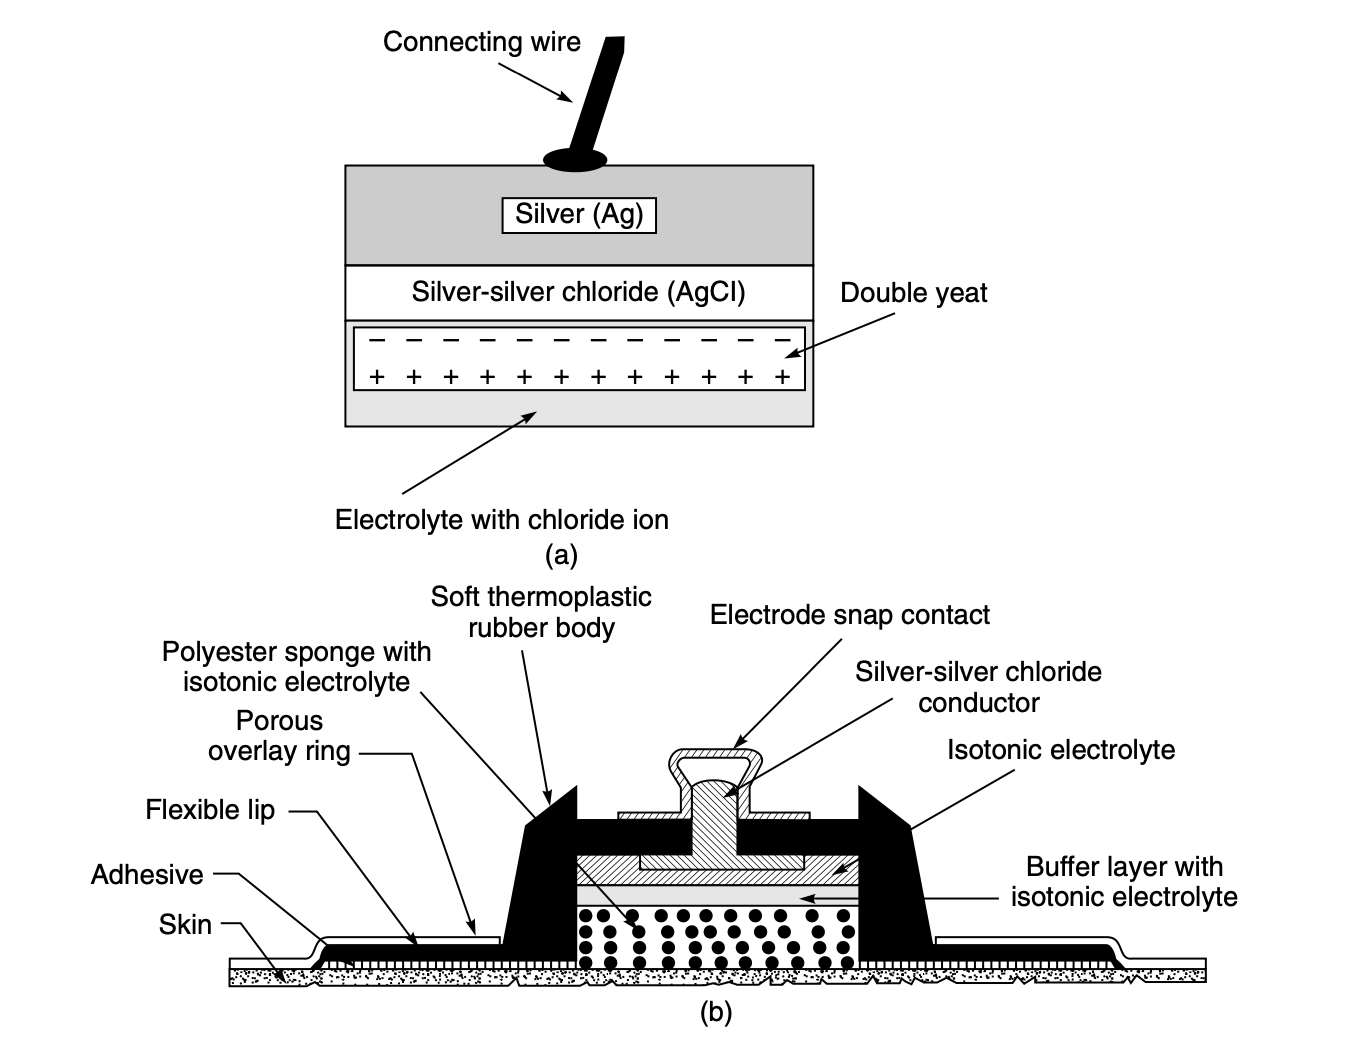
\includegraphics[scale=0.4]{Screenshot 2023-05-01 at 2.27.36 PM.png}
\end{center}
The layer of gel on the electrodes absorbs the possibility of artefacts, drifts and baseline wandering and absorbs the movement to an entirety. The electrodes also reduce the possibility of infection which is a rampant possibility with our basic reusable electrodes. These are also small in size and reduce the time of setting up and removal of the electrode set up. The adhesive used in the electrode should be excessively strong and should have the4 slightest possibility of an unwanted liftoff as it would case damage in readings and is not something we can have while monitoring the characteristics.\\
\\
T5he gel used in the electrolyte should possess the following properties.
\begin{enumerate}
    \item Stay moist for intended shelf life.
    \item Should not be a spot of germination for bacteria.
    \item Provide low impedance.
    \item Should not cause irritation to the person.
\end{enumerate}
The standards which a basic electrode should match before getting approved for clinical usage are found below :
\begin{enumerate}
    \item Direct Current Offset Voltage - A pair of electrodes connected gel-to-gel, after 1 min stabilization period must exhibit offset voltage no greater than 100 mV.
    \item  Combined offset instability and internal noise - $< 150\mu V$
    \item AC Impedance - 10Hz for at least 12 peaks.
    \item Defibrillation Overload Recovery - The absolute value of polarization potential of a pair of electrodes connected gel-to-gel shall not exceed 100 mV, 5s after each of four capacitor discharges. The capacitor should be 10 mF charged to 200 V and discharged through the electrode pair with 100 W in series.
    \item Bias Current Intolerance - The observed dc voltage offset change across an electrode pair connected gel-to-gel shall not exceed 100 mV when subjected to a continuous 200 mA dc current over the period recommended by the manufacturer for the clinical use of the electrodes. In no case shall this period be less than 8 hours.
\end{enumerate}
\subsection{Paste-less Electrodes}
ECG monitoring electrodes, in a majority of the cases, are metal plates applied to the skin after cleaning and application of a coupling-electrolyte in the form of an electrode paste or jelly. Such preliminary preparation can be sometimes irritating and time consuming. Also, it is often not done satisfactorily, resulting in problems like poor quality signals and baseline drift, etc.\\
\\
Another disadvantage of using electrode jelly is that during long-term monitoring there is likely to be patient-skin reactions as the electrode-skin interface dries out in a matter of a few hours. In addition, bacterial and fungal growth can take place under electrodes worn over long periods.\\
\\

\section{Electrodes of EEG}
Most commonly we use a mesh of chlorided silver discs of 6-8mm diameter. The are in contact with the scalp using an electrolytic paste. Sometimes needles are also used to get the EEG but they have to be painfully inserted subcutaneously. \\
\\
Hector (1968) describes a pad electrode which is made from a silver rod belled out at the end and padded with a sponge, or a similar material, contained in gauze. It is screwed into an insulated mount and held in place on the head with a rubber cap. To hold three such electrodes, an adjustable tripod mount is employed. 
\section{Electrode for EMG}
Electrodes for electromyographic work are basically needle types. Needles are essentially used in clinical electromyographic studies, neurography and other electrophysiological investigations. The needles were mostly made of stainless steel and even though it is unfavourable for its noise point of view, it is a natural choice owing to its solidity and low costing. A major factors involved with these needles were autoclave them and sterilising them well before use. Working with needle type EMG setups we run into a basic needle type and a hypodermic needle type of EMG. \\
\\
A new innovation was required in the field of no-invasive surface electrodes for measurement of EMG. The electrode recording surfaces are two concentric steel rings. A third ring attached to the casing of the electrode is the earth contact. The rings are separated from each other by Teflon, the insulating material. The concentric ring instead of the normal passive electrode configuration also obviates the problem of electrode alignment relative to the direction of the muscle fibres. The results of tests undertaken with these electrodes showed that it was able to pick up
individual motor unit action potentials at moderate force levels.
\section{Microelectrodes*}
We need microelectrodes in a condition where we need to check the value of electric signals a cellular level,we run into micro electrodes.\\
There are primarily two types of microelectrodes.
\begin{enumerate}
    \item Metallic Micro-capillaries
    \item Glass Micro-capillaries
\end{enumerate}
\end{document}
